
\documentclass[5p,sort&compress]{elsarticle}

\usepackage{latexsym}
\usepackage{amsfonts,amsmath,amssymb}
\usepackage{url}
\usepackage[utf8]{inputenc}
\usepackage{fancyref}
\usepackage{url}
\usepackage{mathtools}
\usepackage{booktabs}
\usepackage[flushleft]{threeparttable}
\usepackage[english]{babel}
\usepackage[shortcuts]{extdash}
\usepackage{minted}
\usepackage[inline]{enumitem}
\usepackage[labelformat=simple]{subcaption}

\captionsetup[table]{format=plain,labelformat=simple,justification=centering, labelsep=newline, singlelinecheck=false, textfont={sc}}

\bibliographystyle{elsarticle-num-names}

\hyphenpenalty=750
\hbadness=1350
\frenchspacing

\def\topfraction{0.9}
\def\bottomfraction{0.4}
\def\floatpagefraction{0.8}
\def\textfraction{0.1}

\sloppy
\flushbottom

\begin{document}

\begin{frontmatter}
% TODO: Do we want some "organic" title? Growing and stuff?
% perhaps something like this:
% TODO: We need better term than "platform"
\title{Nodewatcher: A Substrate for Growing Your own Community Networks}
%\title{nodewatcher: enabling simple provisioning, deployment and monitoring of community networks}

\author[fri,wlansi]{Jernej Kos\corref{cor}}
\ead{jernej.kos@fri.uni-lj.si}

\author[berkeley,wlansi]{Mitar Milutinović}
\ead{mitar@tnode.com}

\author[fri,wlansi]{Luka Čehovin}
\ead{luka.cehovin@fri.uni-lj.si}

\cortext[cor]{Corresponding author}

\address[fri]{University of Ljubljana, Faculty of Computer and Information Science, Ljubljana, Slovenia}

\address[berkeley]{University of California, Berkeley, USA}

\address[wlansi]{wlan slovenia, Open wireless network of Slovenia, \url{https://wlan-si.net}}

\begin{abstract}
TBD.
\end{abstract}

\begin{keyword}
community networks \sep provisioning \sep monitoring \sep deployment \sep management \sep wireless \sep mesh
\end{keyword}
\end{frontmatter}

\section{Introduction}

Community (wireless) networks \cite{Bruno_2005} provide independent, community-owned network infrastructure for user communication and data exchange.
They are mostly built by using standard wireless (IEEE802.11) ad-hoc infrastructure \cite{Akyildiz_2005}, by laying own optical fiber and, more recently, by the use of free-space optical systems \cite{Mustafa_2013}.
Their common aim is to empower people with new ways of communication and access to the wider public networks like the Internet while preserving autonomy from large service providers and other parties.
The importance of community networks has also been recognized for enabling large scale scientific experiments in real-world networks by project CONFINE~\cite{Braem_2013}.

The common property of all community networks is that they grow organically~-- there is no central planning that would decide how the network is built, as is usually the case with commercial networks.
Instead, the network grows in a bottom-up fashion as more people express interest in participating in the community and connect with their neighbours.
Because of this growth pattern and community involvement, management of such networks presents some unique challenges:

\begin{itemize}
\item In most of the community networks, people who maintain the network infrastructure are volunteers with limited free time that they can spend on network management.
This makes efficient management very important for network growth.

\item There are many repetitive tasks in community network operation, especially related to configuration, deployment and monitoring of network equipment.
Without a suitable overall management system, all these steps (flashing and configuring devices, allocating resources, diagnosing problems) need to be done manually which is time-consuming and prone to errors.

\item In addition to technical issues related to device deployment, there is also the need for community coordination so that people know what is going on in the network and can familiarize themselves better with its operation and what others are doing.
\end{itemize}

Various solutions have appeared in an attempt to address these challenges~-- as we will show, each community developed its own model of operation with its own accompanying set of tools.
The problem with this approach is that work is being duplicated for every new community network and that these various solutions are mostly not interoperable between each other.
So why would new communities not reuse existing tools?
The problem lies in the fact that these tools have not been built to be customized to the needs and operation of individual communities.
Each community has at least slight differences in their vision and operation philosophy and this requires customization on several fronts, to only name a few:
\begin{enumerate*}[label=\itshape\alph*\upshape)]
\item different routing protocols may be used;
\item some communities use VPN tunnels to establish certain long-range links using different protocols;
\item network topologies may differ among communities, some use central clusters of nodes as gateways to peer with other networks, some use a more distributed topology;
\item some communities attach various sensors to nodes and would like to monitor their outputs through time;
\item there may be differences in operation due to local regulations.
\end{enumerate*}

In order to address this, there are at least two approaches that can be taken.
The first approach is to try to create a common system that addresses the needs of as many of communities as possible by providing a large feature set and a large configuration schema encompassing all possible scenarios.
This approach has been tried as part of an interoperability effort [?] established between community networks, to come up with a common schema upon which so called node databases could be built.
The problem is that it is hard to come up with a one-fits-all solution and large monolithic schemas can quickly become unmanageable.

The other approach is to create a minimal core, but to make it completely modular and extensible at multiple points so that community networks can tailor it to their needs, whatever they might be.
This is the approach that we are taking with the nodewatcher v3 platform.
We make the following novel contributions:
\begin{itemize}
\item A modular open platform that may be easily tailored to the needs of any community network.
\item An extensible per-node firmware image generation module that enables generation of pre-configured images for specific nodes in order to eliminate any manual configuration requirement on the nodes.
\item An extensible monitoring system module with a scalable time-series data storage backend enabling large-scale collection of status and other telemetry data while supporting interactive visualizations.
\end{itemize}

The rest of this paper is organized as follows.
Section~\ref{sec:related-work} presents related work done in the area of community network management tools.
Section~\ref{sec:platform} presents the design and functioning of the nodewatcher platform.
Section~\ref{sec:evaluation} shows the results of platform evaluation in the wlan slovenija community wireless network.
Section~\ref{sec:conclusion} presents conclusions and ideas for future work.

\section{Related Work}
\label{sec:related-work}

There exist several proposals on how to manage networks, traditional and community ones.
We survey them in this section and show contrasts with our platform.

\subsection{Node Databases}

Many wireless mesh network communities have quickly recognized the need for having a central system that would be able to manage the multitude of wireless mesh nodes.

One of the oldest and largest mesh networks are Guifi.net \cite{Guifi_2003,Vega_2012} and the \textit{Athens Wireless Metropolitan Network} with its WiND \cite{AWMN_WIND_2002} (Wireless Node Database).
As the node database solutions evolved with the network, both are tailored to specific structures of their respective networks and its management structure.
% TODO

- Freifunk FFM/CWNOS \cite{Funkfeuer_2012}
- Nodeshot \cite{Nodeshot_2012}

\subsection{Traditional Network Management}

- Traditional network management systems?

\subsection{Modular Platforms}

Trac as an example of modular system for managing open source projects.
Trac Hacks. -> Same for networks.

\section{Platform}
\label{sec:platform}

\subsection{Overview}

\begin{figure}
  \centering
  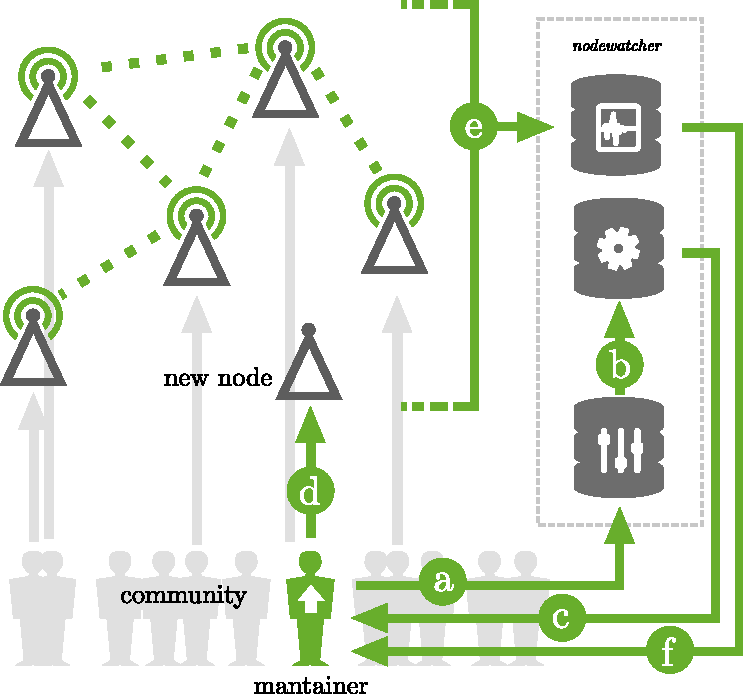
\includegraphics[scale=0.4]{figures/device-mgmt-cycle.pdf}
  \caption{Device management cycle illustrating how devices are managed in a community network.
Traditionally the configuration, generation and monitoring steps are performed manually, while the nodewatcher platform enables automation of these tasks, freeing up resources inside a community.}
  \label{fig:device-mgmt-cycle}
\end{figure}

% TODO: Po mojem bi morali tu dati nekje tudi cloveka v diagram. Ker sicer izgleda tako tehnicno. V smislu, ce je community network, kje je community v tem ciklu?

The core idea behind the nodewatcher platform is the \textit{device management cycle}, illustrated by Figure~\ref{fig:device-mgmt-cycle}.
The cycle starts with the \textit{configuration stage} where devices are configured for use in a specific location in the network.
At this stage, device configuration is still platform-independent and does not depend on the hardware that will be later used to deploy the device.
The latter only happens in the next stage, the \textit{generation stage}, where platform-independent configuration is transformed to device- and platform-specific configuration.
For easier deployment, a firmware image for the target device may also be generated.
In the \textit{deployment stage}, configuration or firmware is applied to the target device and the device is deployed in the field.
As soon as the device is deployed and is able to join the network, it is monitored by the platform.
In the \textit{monitoring stage}, the device is actively monitored for correct operation in context of the whole network.
In case errors in configuration or other problems are detected, the device's maintainer is notified so the device may be fixed and/or reconfigured, repeating the cycle.

The nodewatcher platform aims to provide components for all stages of the described device management cycle.
Each part is designed to be easily extensible to networks with various topologies, routing protocols, operating systems and hardware devices.
In the next sections we will describe the network management platform components in detail.

\subsection{Platform-independent Configuration}

Community networks are usually built from a wide range of devices, containing everything from off-the-shelf home routers to specialized devices used for backbone links and regular servers used for core services.
The nodewatcher platform uses a single platform-independent schema to describe configuration for all these types of nodes, regardless of their hardware and/or operating system.
One of the motivations behind this choice is that platform-independent configuration enables replacement of devices without the need to do much re-configuration.
It is a frequent occurrence that deployed devices need to be replaced when they stop functioning properly due to various hardware failures.

However, while having a platform-independent configuration, some configuration properties depend on features which are inherently device-dependent (for example the number of ethernet ports, available wireless radios, supported protocols, etc.).
In such cases the user editing the platform-independent configuration may create a configuration which will fail to work when applied to the target device.
This can either further delay problem discovery until the \textit{deployment} stage when it is already too late and costly to fix problems, especially in wireless networks where nodes may be deployed in hard-to-reach locations.
This clearly shows the need to have instant validation and feedback (the \textit{feedback} arrow in Figure~\ref{fig:device-mgmt-cycle}) when updating platform-independent configuration.
This validation must be based on the selected target device with all its hardware and software properties.
The nodewatcher platform enables such instant validation, which is handled by the firmware generator component (see Section~\ref{sec:firmware-generator}).

In the introduction we mentioned the problem with attempting to design an all-encompassing schema or a single node database application that would cover every possible deployment of community networks.
Communities will usually have some specifics regarding their operations~-- either because of different local regulations or differences in philosophy.
Having a single unified schema can quickly become a limiting factor and things need to be worked around it in order to adapt the solution for the local community.

\begin{figure}
\centering
\begin{minted}[fontsize=\small]{python}
class VIFConfig(InterfaceConfig, RoutableInterface):
  device = registry_fields.IntraRegistryForeignKey(
    WifiRadioDeviceConfig, null=False,
    related_name='interfaces'
  )

  mode = registry_fields.RegistryChoiceField(
    'node.config', 'core.interfaces#wifi_mode')
  essid = models.CharField(max_length=50,
    verbose_name="ESSID")
  bssid = registry_fields.MACAddressField(
    verbose_name="BSSID",  blank=True, null=True)

# Register schema item into the schema which makes it
# available to any other module.
registration.point('node.config').register_subitem(
  WifiRadioDeviceConfig, VIFConfig)
\end{minted}
\caption{An example of a platform-independent schema definition for a virtual wireless interface configuration.}
\label{fig:schema-module-wifi}
\end{figure}

The nodewatcher platform avoids this problem by making the platform-independent schema itself completely extensible.
It is the individual modules that may register schema items and the final schema is the union of all these items.
An example of such a schema item definition is shown in Figure~\ref{fig:schema-module-wifi}, where several properties of the schema extension mechanism can be shown:
\begin{itemize}
    \item The schema items are class-based, which means they can be extended later on by other modules (in the example the \texttt{VIFConfig} extends a more generic \texttt{InterfaceConfig} which may be provided by another module).
    \item Fields that represent enumerations (in the example \texttt{mode} is such a field) do not hardcode the possible options, but only provide an \textit{extension point} where additional choices can later be registered by other modules.
    Each such extension point is attached to a unique name (e.g. \texttt{core.interfaces\#wifi\_mode}) that may be referenced later when extending it.
    \item Schema items may reference other items (in the example, \texttt{device} references the parent radio device that this virtual wireless network configuration is being configured on).
\end{itemize}

To construct the base schema that is available with the nodewatcher platform, we have surveyed all the different solutions mentioned in Section~\ref{sec:related-work} and included a small amount of items common to most of the communities.
But even these base items of the schema are just module registrations which makes them removable in case some community needs to really change how things work.

The system that supports such schema item registrations is called the \textit{registry} and is essentially a lightweight extension of the standard object-relational mapper (ORM) concept~\cite{ONeil_2008} as the mentioned schema items are actually models.
The problem that it aims to solve is the one of simplified model discovery. In an extensible platform like nodewatcher, modules may want to query on fields defined by other modules somewhere in the schema. For example, there is an item called \texttt{GeneralConfig} in the base schema, enabling users to configure a \texttt{name} for a node:

\begin{minted}[fontsize=\small]{python}
class GeneralConfig(NodeConfigRegistryItem):
  name = models.CharField(
    max_length=30,
    null=True,
    validators=[core_validators.NodeNameValidator()],
  )
\end{minted}

This base item does not provide any other fields besides the node name, leaving potential extensions to other modules.
Let us now say that we would like to also add a choice field which would specify what device is in use on a specific node. We may do that in another module by saying:
\begin{minted}[fontsize=\small]{python}
class ExtendedConfig(GeneralConfig):
  device = registry_fields.RegistryChoiceField(
    'node.config', 'core.general#device', blank=True)
\end{minted}

Imagine now a module that would like to perform a query listing only nodes that use a device called \texttt{tp-wr741ndv4}.
As mentioned, these two classes actually represent ORM model definitions so a traditional query traversing these two relations would go something like:
\begin{minted}[fontsize=\small]{python}
Node.objects.filter(
  generalconfig__extendedconfig__device='tp-wr741ndv4'
)
\end{minted}

Here we make the assumption that there is a one-to-one relation between node and \texttt{GeneralConfig}.
While one-to-many relations are also supported (so each node can have multiple instances of a model), we limit ourselves to this simple case for ease of exposition.
Note how even in this very simple example we had to explicitly specify the hierarchical path that is spanning these two relations.
This makes such a method not very developer-friendly under the requirement of extensibility and even more complex schemas.
One of the features that the registry enables, is that we can simplify the same query as:
\begin{minted}[fontsize=\small]{python}
Node.objects.registry_filter(
  core_general__device='tp-wr741ndv4'
)
\end{minted}

In this case, the \texttt{core.general} is the \textit{registry identifier} that is attached to the base model and represents itself or any of its subclasses at the same time.
In the background, the proper relations are automatically deduced and the query executed.
Similar extensions are also provided for simplified fetching of fields deeply nested in the schema.

\subsection{Form Generation and Rule-based Defaults}


- another important issue to address is how to specify defaults so users can quickly get working configurations for some common use cases; rules engine?

\subsection{Resource Allocation}

As in any network, there is also a need to perform IP address resource allocation in community networks.
This is especially the case in IPv4-based networks where it is hard to automatically generate node addresses without collisions due to the small available space.

%TODO citation for buddy allocation scheme
In order to support that, nodewatcher implements a hierarchical buddy allocation scheme [?] extended with support for hold down timers.
At the top level IP space is split into multiple pools from which other objects (for example nodes) may request specific allocations.
Hold down timers are necessary to avoid collisions with nodes that have been recently removed.
When an allocation is freed, it is still marked as \textit{reserved} until the hold down timer expires.

This is required especially in community networks where nodes may not be completely removed and may actually reappear at a later time, causing routing conflicts.

\subsection{Firmware Generator}
\label{sec:firmware-generator}

\begin{figure*}
  \centering
  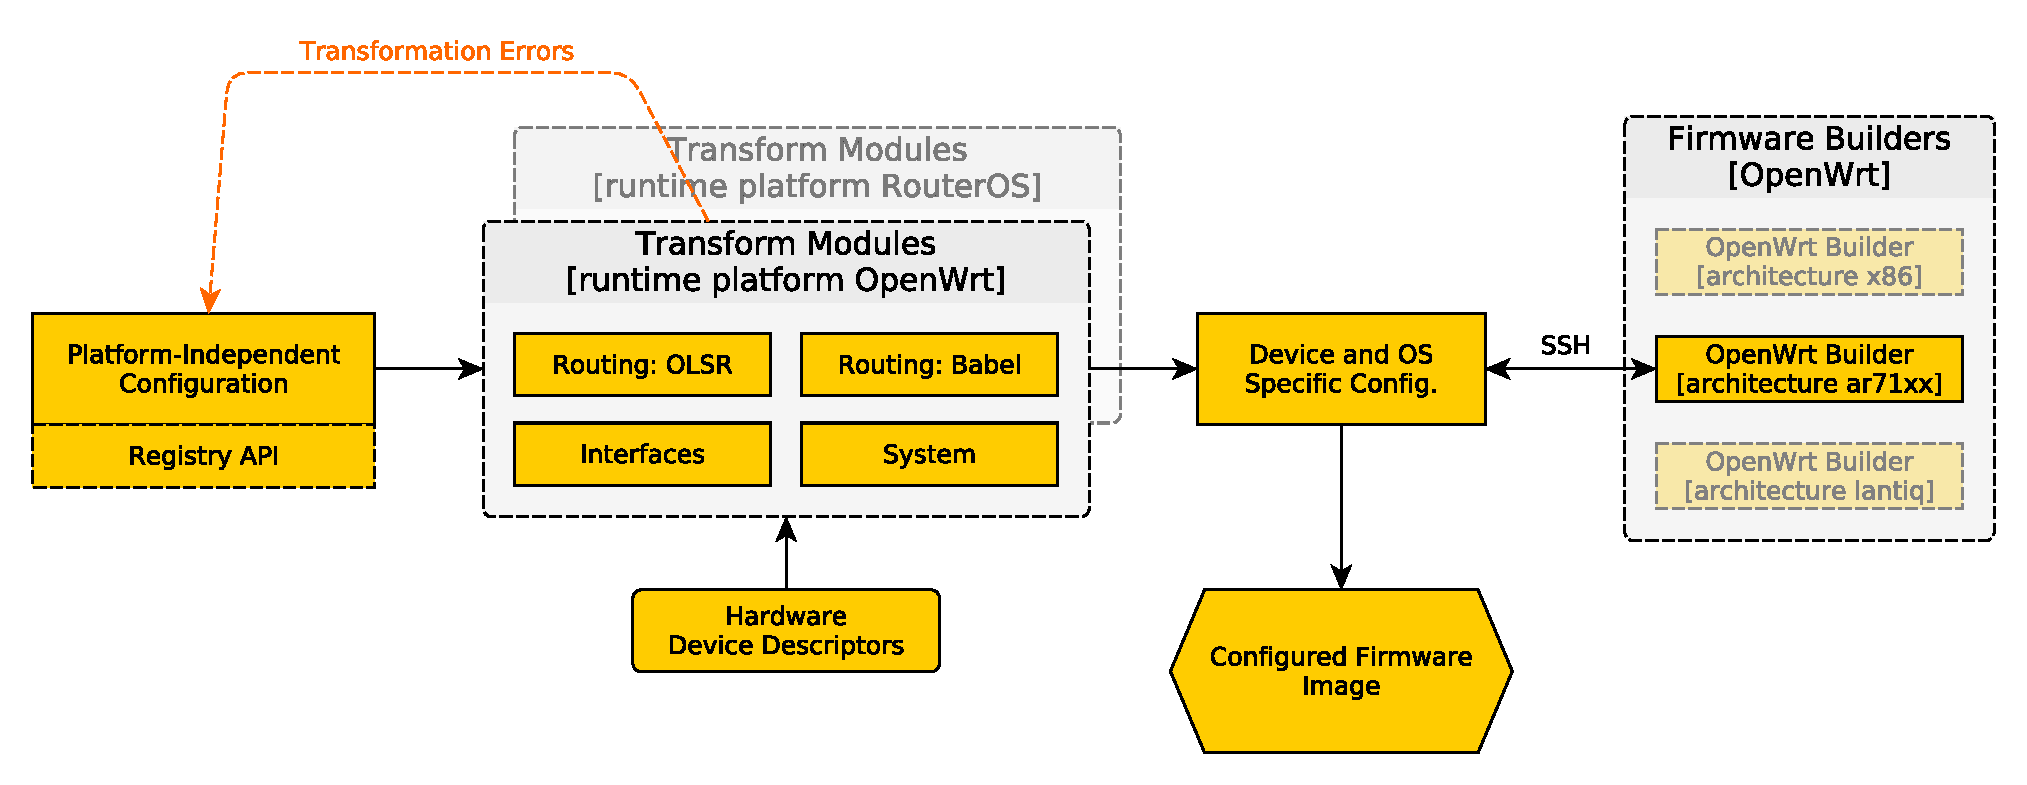
\includegraphics[scale=0.5]{figures/firmware-buildsystem.pdf}
  \caption{An overview of the firmware build system, coming from platform-independent configuration in the first stage to the fully configured firmware image that may be flashed directly onto the target device in the final stage.
The firmware builders are Docker containers with pre-built firmware build toolchains.}
  \label{fig:firmware-build-system}
\end{figure*}

Traditionally, devices may be configured manually before they are deployed.
This is usually done either through a command-line interface via SSH or a graphical user interface via HTTP, depending on the firmware running on the device.
In both cases, however, this is an error-prone process due to manual user input.
Mistakes can easily happen and sometimes they might propagate to the deployment stage where they are hard and costly to fix.
In community wireless networks, devices are sometimes deployed in hard-to-reach locations like rooftops or high towers and fixing certain problems requires physical access to the device.

As described, the nodewatcher platform can be used to store device configurations in a platform-independent way.
But this configuration cannot directly be used on devices.
Different operating systems like the open source OpenWrt [?] or the proprietary RouterOS [?] that are usually used on devices in community networks, have completely different ways of being configured.
This is why an additional platform-dependent transformation step is needed.

However, such a step presents some additional challenges that prevent a straightforward transformation of any configuration based on the platform-independent schema to a device-specific one.
This is due to the fact that there are differences between operating systems which may prevent certain configurations from being properly instantiated on one operating system even when those same configurations work without issues on another one.
Additionally even using the same operating system, devices have different capabilities due to differences in their hardware.
Configuration which was platform-independent and unaware of the target device in the first stage can produce problems while being applied to a specific device and operating system.
This conflict may result in some unpleasant, but realistic, scenarios:
\begin{enumerate}[label=\roman*)]
\item Devices have different default network switch layouts and VLAN tags.
As usually nodes use the WAN-designated port for the internet uplink and the LAN-designated port for routing to nodes in the same location, such a misconfiguration will cause connectivity issues.

\item Configuration of some wireless authentication mechanisms requires the installation of specialized packages on some operating systems.
Without them even a valid configuration will simply not work.

\item Different devices have different radio capabilities.
For example, some devices only support IEEE802.11a channels and if the configuration system is not aware of this, blind configuration transformation to the target platform results in a failure to bring up the wireless device.
\end{enumerate}

These scenarios show that supporting informed decisions of the configuration transformation process requires the use of a device database component.
Nodewatcher takes a declarative approach to device descriptors which enumerate all the hardware and software properties of a given device:
\begin{minted}[fontsize=\small]{python}
class TPLinkWR741NDv1(cgm_devices.DeviceBase):
  identifier = 'tp-wr741ndv1'
  name = "WR741ND (v1)"
  manufacturer = "TP-Link"
  url = 'http://www.tp-link.com/'
  architecture = 'ar71xx'
  radios = [
    cgm_devices.IntegratedRadio('wifi0', "Wifi0", [
      cgm_protocols.IEEE80211BGN(
        cgm_protocols.IEEE80211BGN.SHORT_GI_20,
        cgm_protocols.IEEE80211BGN.SHORT_GI_40,
        cgm_protocols.IEEE80211BGN.RX_STBC1,
        cgm_protocols.IEEE80211BGN.DSSS_CCK_40,
      )
    ], [
      cgm_devices.AntennaConnector('a1', "Antenna0")
    ], [
      cgm_devices.DeviceRadio.MultipleSSID,
    ])
  ]
  switches = [
    cgm_devices.Switch(
      'sw0', "Switch0",
      ports=5,
      cpu_port=0,
      vlans=16,
    )
  ]
  ports = [
    cgm_devices.EthernetPort('wan0', "Wan0"),
    cgm_devices.SwitchedEthernetPort(
      'lan0', "Lan0",
      switch='sw0',
      vlan=1,
      ports=[0, 1, 2, 3, 4],
    )
  ]
  antennas = [
    cgm_devices.InternalAntenna(
      identifier='a1',
      polarization='horizontal',
      angle_horizontal=360,
      angle_vertical=75,
      gain=2,
    )
  ]
  # Configuration below this point describes
  # differences for each supported operating
  # system (in this case 'openwrt').
  port_map = {
    'openwrt': {
      'wifi0': 'radio0',
      'sw0': 'switch0',
      'wan0': 'eth1',
      'lan0': 'eth0',
    }
  }
  drivers = {
    'openwrt': {
      'wifi0': 'mac80211'
    }
  }
  profiles = {
    'openwrt': {
      'name': 'TLWR741',
      'files': [
        'openwrt-ar71xx-generic-tl-wr741nd-v1.bin'
      ]
    }
  }
\end{minted}

Device descriptors may be subclassed in order to simplify definitions of new devices with only slight variations.
This feature greatly improves the time to fully support new devices which is important in the quickly evolving community networks.

Using these device descriptors and the platform-independent configuration provided in the first stage, nodewatcher is able to generate device-specific configuration using a transformation step (see Figure~\ref{fig:firmware-build-system} for an overview of the whole process).
The transformation step is built by a pipeline of modules where each of them gets the platform-independent configuration as input and may produce modifications to the device-specific configuration as its output.
Such a modular transformation step ensures that the pipeline can be adapted to a wide range of transformations (for example, supporting various routing protocols, sensor inputs, network configurations etc.), so everything that a target device and operating system support may be used.
Recalling the importance of the feedback arrow in Figure~\ref{fig:device-mgmt-cycle}, the transformation module pipeline may also raise errors when parts of the input configuration could not be properly transformed.
These errors are immediately propagated up to the user who is entering configuration via the nodewatcher's web interface, so that problems may be corrected as soon as possible.
The validation system will not save a configuration which has outstanding errors, preventing invalid configurations from being used to deploy devices.

In order to further ease deployment, the resulting device-specific configuration may be packaged together with a firmware image which may be then flashed directly onto the target device.
Such pre-generated firmware images further reduce the room for errors as no configuration needs to be transferred separately or entered manually.
Besides reducing errors, packaging software (firmware) together with its configuration is also beneficial for ensuring that the configuration really is applicable to the used software versions as both can be tested together.
Otherwise, using a stale configuration on a newer operating system or newer versions of some packages may result in failing devices.
Bundling firmware together with node-specific configuration is a novel way of provisioning devices in community networks  that would be beneficial to existing and emerging networks.

The underlying firmware build system has been built in such a way that it is extensible to different operating systems and platforms.
To achieve this, the build system is structured into multiple Docker containers~\cite{Docker_2013}.
Docker containers are a lightweight wrapper around the Linux namespacing API and filesystem layers with a goal to enable an interface for packaging applications in a reusable and extensible way.
Namespaces provide container isolation (the containers still share the host kernel), so that adjacent containers running on the same host are unable to see or influence each other's processes, network configuration, etc.
Each container can be thought of as a very lightweight virtual instance, but without the overhead of running a full virtual machine with its own kernel.
Nodewatcher uses the Docker container features in order to generate and run firmware image builders for multiple platforms.
The build process is specific for each operating system and currently only OpenWrt is supported as it runs on the most devices that are in use in community networks.

When the device-specific configuraion has been generated by the transformation step (see the central node in Figure~\ref{fig:firmware-build-system}), a suitable builder is selected based on the architecture and software platform specified in the device descriptor.
After a builder is identified, the nodewatcher process establishes a secure shell (SSH) connection to the selected container, transfers the configuration there and starts the build process which completes in a matter of seconds.
This decoupling of configuration and actual builders enables the builder containers to be actually deployed on another machine with more resources.

By packaging firmware builders as containers, nodewatcher enables simple reuse and sharing of ready-made builders between community networks.
Compiling and preparing a range of firmware builder toolchains can be a lengthy process requiring manual configuration, but such containerized organization enables communities to simply download pre-built toolchains and use them in their nodewatcher instances without compiling anything.

The described system is also extensible -- adding support for new architectures simply requires a new builder container to be prepared, while adding support for new operating systems also requires an extension of the configuration transformation process.

\subsection{Network Monitoring}

- a nice figure showing how data flows from the devices via the nodewatcher-agent via http/json to the monitor process and then is stored via datastream
- nodewatcher-agent
  - runs on OpenWrt
  - supports various data reporting via an extensible JSON schema
  - modules may evolve their schema independently from others (schema versioning)
- backend processing architecture (monitord)
  - enables constructions of arbitrary processing pipelines
  - supports automatic parallelization of operations based on the constructed pipeline

\subsubsection{Time-series Data Storage}

- storing everything that is going on in a large community network represents a lot of data
- downsampling, parallelization
- support for later seamless interactive visualization

\subsection{Easy-to-use User Interface}

TODO

notifications
easy to debug
easy to share information about nodes
information keept to date

strict-typing - compiling until there is no errors - you can start with basic router installation and system will be telling you what is wrong and how to fix it and when you fix all errors, you get a working node

but you can also install it through generator

TODO

should we extract some code into external packages like registry and then describe them (registry, datastream, template-overload)?

\section{Evaluation}
\label{sec:evaluation}

TODO

- we should show how an actual deployment looks like in wlan slovenija (a nice schematic figure)
- wlan slovenija, v2, experiences?
- performance comparison, v2 vs. v3?

\section{Conclusion and Future Work}
\label{sec:conclusion}

TODO

- radio planning features

\section*{Acknowledgement}

The authors have been supported by the following institutions: Jernej Kos by the Slovenian Research Agency (Grant 1000-11-310153), by the Shuttleworth Foundation Flash Grant and by the NLnet Foundation (Grant 2014-05-015).

\section*{References}
\bibliography{bibliography/references.bib}

\end{document}
